\chapter{Dominant points}
In shape analysis, extracting features from the curves is an important step because in another way, we can re-construct the shape from the features. The term dominant points, also called as siginficant points, points of interest, corner points or landmarks is assigned to the points which have the high effect on boundary of object; their dectection is a very important aspect in contours methods because these concentrate the information of a curve on the shape.\\[0.2cm]
Dominant points can be used to produce a presentation of a shape contour for futher processing. The representation ...
In the content of this chapter, we will discuss about the methods to determine the dominant in digital image.\\[0.2cm]
There are many approaches developed for detecting dominant points and the methods can be classified into three groups follows:
\begin{itemize}
	\item Dectermine the dominant points using some significat measure other than curvature
	\item Evaluate the curvature by transforming the contour to the Gaussian scale space.
	\item Search for dominant points by estimating directly the curvature in the original image space.
\end{itemize}
\section{Hough Transform}
One of the challenges in image processing is detecting the characteristic of the object for recognition. Shape recognition is done by searching or detecting a class of simple geometric object such as line, curves in the image and comparing with the model. The matching score of the shapes is calculating by a measurement distance (such as Bhattacharyya). Instead of comparing between the geometric classes from the shapes, we can detect the presence of a shape in anther shape by searching each feature of the shapes. To sovle this problem, Hough Transform (HT)\cite{mukhopadhyay2015survey} is varied. At the beginning, HT\cite{vc1962method} is used to detect the line. It converts the space of parameters from x and y (coordinate of points in line) to space of slope and y-intercept of the line by voting process. For each object statisfying with equation of a line, it votes for the bin have correspondence slope and y-intercept. The set of bins is called the accumulator.
\subsection{Generalizing Hough Transform}
Until now, HT is still a good method for line detection or object recognition. But one of the weakness of HT is cannot determine the end points of the line segments. For this reason, the Generalized Hough Transform (GHT), introduced by Ballard\cite{ballard1981generalizing} is a generalization of HT to detect non-parametric curves. The process includes two phases: learning and recognition. In learning phase, a R-table is construct for model object. R-table is constructed based on the geometric information of each points in curves of object model with a reference point. The reference point can be arbitrary point in the model. Each row in R-table includes the gradient direction of each point which was chosen as index of table; and the polar coordinate values of each point. This mean that a gradient direction can be having many polar coordinate values. During recognition phase, an accumulator is created, called Hough Space. For each point in the scene object, finding the correspondce gradient direction in the R-table and voting at all the coordinate values. The peak in accumnulator is position of reference point of the model object in the scene object. And the peak value is equal to the number of boundary points of the object  when the model and the scene match perfectly.\\[0.2cm]
During recognition phase, the translation and rotation between model object and scene object is determine by principal component axis. Based on the curve points of the object, the centroid of each object is calculated. Then, the principal axis of each object is indicated. The translation between two objects is difference of two centroid points. The angle to rotate is the angle difference of two axes.\\[0.2cm]
When model and scene are matching, the dominant points (landmarks) of scene object is estimated from landmarks of model object by applying the translation, rotation from the centroid points. The last result is verifying by apply template matching (which will discuss as section \ref{template}).
\subsubsection{Result}
Using GHT to extract the landmarks on beetle is experiment on 287 images of right mandible of beetle. To compare the matching between the location of manual landmarks and estimated landmarks, the centroid size is compute for each set of landmarks.\\[0.2cm]
\begin{figure}[h!]
\centering
\subfloat[Model 28]{\label{figcentroidSize1}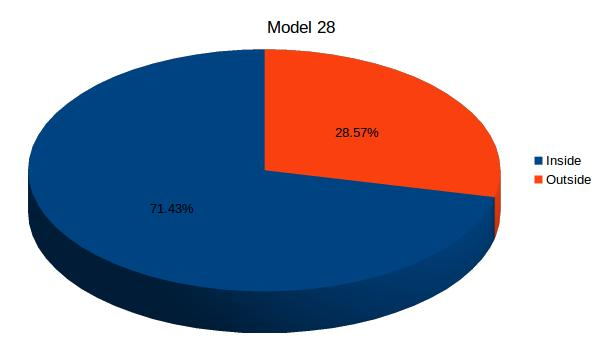
\includegraphics[width=0.5\textwidth]{./images/cmodel28}}~~
\subfloat[Model 71]{\label{figcentroidSize2}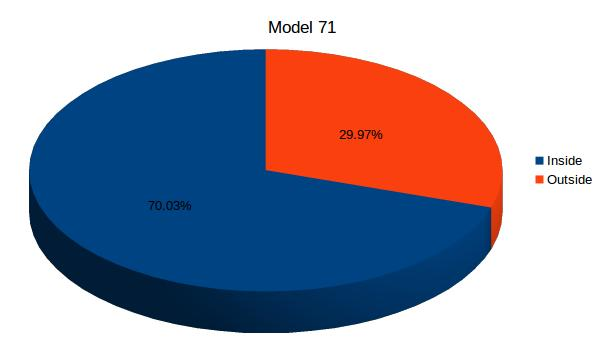
\includegraphics[width=0.5\textwidth]{./images/cmodel71}}
\caption{The accuracy of centroid size on mandible}
\label{figcentroidSize}
\end{figure}
Figure \ref{figcentroidSize} display the accuracy of the centroid size of estimated landmarks when we compare with the centroid size of manual landmarks. We use 2 images (Md28.JPG and Md71.JPG) as model. The number of landmarks be detected on scene object is 100\%. For model 28, 71.43\% the centroid of estimated landmarks is placed inside the standard deviation (SD) of manual landmarks, 28.57\% is outside the SD. The ratio for model 71 are 70.03\% and 29.97\%.
\subsection{Probabilistic Hough Transform}
To speed up Hough Transform, instead of processing on all data set, we can consider a subset of data points. The popular method is  \textbf{Probabilistic Hough Transform}. Probabilistic Hough Transform (PHT) is used to detect the presence of a model image in a scene image based on the group of features. The hypothesised location of the model image in the scene image is indicated based on the conditional probability that any pair scene lines agreement about a position in model image. Applying PHT can be separated into two steps: firstly, recording the information of model image and try to find the presence of the model image in scene image (called training process); secondly, predicting the pose of model image in the scene image (called estimating process).\\[0.2cm]
During training process, choose an arbitrary point in the model image, called reference point. For each pair of lines in model image, the perpendicular distance and angle from each line to reference point is recording (angle is calculated as angle between line and a horizontal line begin from reference point). The presence of model image in scene image is detected by PHT with \textit{``vote"} procedure. Finally, we choose the similar pair lines between model image and scene image. The chosen pair is obtained from best \textit{vote} when we consider each pair of line in scene image with each pair of lines in model image.\\[0.2cm]
In estimating process, the reference point in model image is estimated in scene image by extending the perpendicular lines of the pair of scene lines at the appropriate position. There, we can estimate the pose of the model in the scene image.

\section{Template matching}\label{template}
Template matching is a technique for finding areas of an image that match to a template image (template) by sliding the template over each pixel on the image (commonly cross-correlation). At each position, the sum of products between two images is calculated. The position is considered similar if the sum value at this position is maximal. The equation of cross-correlation is as follows:
\begin{equation}
\label{eq:cross-correlation}
	R_{ccorr}(x,y) = \sum\limits_{x',y'}[T(x'.y').I(x + x', y + y')]
\end{equation}
Where:
\begin{itemize}
\item T is template which use to slide and find the exist in other image.
\item I is image which we expect to find the template image
\item $(x', y')$ are coordinates in template where we get the value to compute.
\item $(x + x', y + y')$ are coordinates in image where we get the value to compute when template $T$ sliding.
\end{itemize}
However, if we use the original image to compute and find the similarity, the brightness of the template and the image might change the conditions and the result. So, we can normalize the image before applying the cross-correlation to reduce the effect of lighting difference between them. The normalization coefficient is:
\begin{center}
\begin{equation}\label{eq:normalizeCoff}
Z(x,y) = \sqrt{\sum\limits_{x',y'}T(x'.y')^{2}.\sum\limits_{x',y'}I(x + x', y + y')^{2}}
\end{equation}
\end{center}
The value of this method when we normalized computation as below:
\begin{center}
\begin{equation}\label{eq:cross-correlation}
R_{ccorr\_norm}(x,y) =\frac{R_{ccorr}(x,y)}{Z(x,y)} = \frac{\sum\limits_{x',y'}[T(x'.y').I(x + x', y + y')]}{\sqrt{\sum\limits_{x',y'}T(x'.y')^{2}.\sum\limits_{x',y'}I(x + x', y + y')^{2}}}
\end{equation}
\end{center}
\section{Image registration}
Image registration is process of transforming difference data sets into the same space and comparing or integrating the data from them. The object in image registration may be the images, time series or viewpoints. It is having many application in medical, military or satellites. In recent years, image registration is applied for both 2D and 3D objects with many methods. These methods may be classified following the characteristics of the input such as \textit{intensity-based and feature-based}, \textbf{transformation}, \textit{spatial and frequency},... In the context of this section, we want to discuss around the methods of linear transformations which include rotation, translation and scaling. Besides, we use these method to generate the general model from several objects or detect the landmarks on the object.
\subsection{Principal component analysis (PCA)}
Principal component analysis is computed based on principal directions of the datasets (model and scene). The input of this method is the list of points on curves of model and scene object (called model points and object points). The origin of the axes is centroid of all points on the curves. One of the axes is the line over the origin and having the minimum distance to all points in the curves; another axis is perpendicular axis with the first axis. The translation between two objects is different distance of centroid point coordinates; the rotation is different angle of two coordinate systems. The steps in PCA are followed:
\begin{itemize}
	\item Compute the centroid of model and scene object,
	\item Calculate the principal axes of model and scene,
	\item Compute the translation and rotation
	\item Translate the model to the scene that they have the same centroid.
	\item Rotate the model followed the different angle to match with the scene.
\end{itemize}
\subsubsection{Result}
The method is experiment with the set of right mandibles. Most of model can be detected its position on the scene by PCA. It also determine the translation and rotation information (see figure \ref{figpca1}). But in the case the input has more the noises, the centroid may be missed with correct position, following it is wrong translation and rotation(see figure \ref{figpca2}). In these examples, the red line is presented for the scene object and blue points is presented for the model object, which we want to align with the scene.
\begin{figure}[h!]
\centering
\subfloat[PCA with less noises]{\label{figpca1}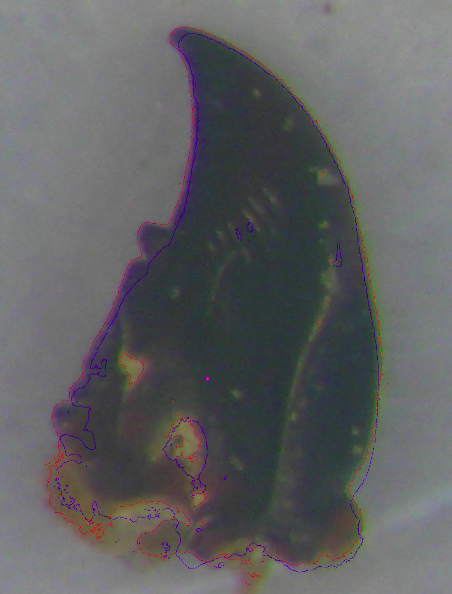
\includegraphics[width=0.3\textwidth]{./images/pca1}}~~
\subfloat[PCA with noises]{\label{figpca2}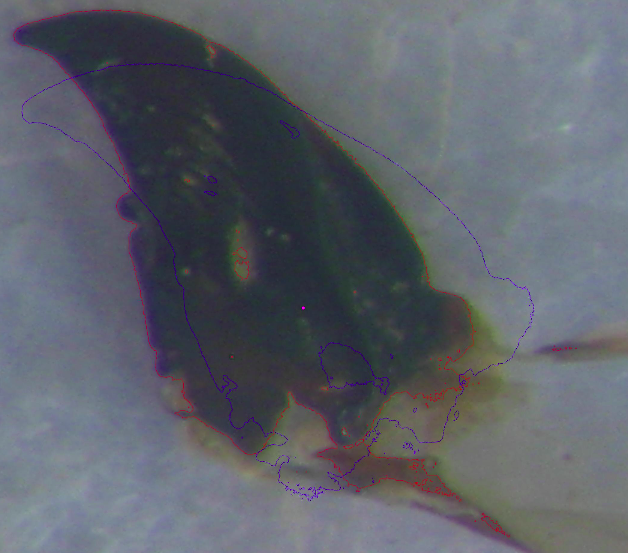
\includegraphics[width=0.4\textwidth]{./images/pca2}}
\caption{The result after applying the PCA}
\label{figpca}
\end{figure}
\subsection{PCA Iteration (PCAI)}
PCA method is a simplest method to align two images. However, PCA is more influenced by noises(see figure \ref{figpca}). Based on the idea of PCA method, PCAI try to apply the PCA on the interested data of the input.\\[0.2cm]
The solved problem in PCAI is the same with other difference registration methods. With two set of data input, specify curve points, we want to register two images with best matches. In PCAI method, firstly, PCA is applied on all two set of data for having the first sight of data. Secondly, the data is sorted followed one of coordinates of data points. The interested data is taken up with a half of data points which are sorted. Thirdly, an iteration will be executed to match the data. For each iteration, we re-compute the principal component of scene data and compare with the model. The iteration will be terminated when the difference position between two images is smallest.\\[0.1cm]
Beside applying PCAI to make the images are matched. PCAI can combine with other technique to estimate the landmarks, such as template matching. At beginning, PCAI is applied to match the images. At the end, for each manual landmarks on the model, we apply the template matching to estimate the location of landmarks on scene image. 
\subsubsection{Result}
The combining between PCAI and template matching is experimented on two datasets of mandible (left and right mandible). For each set of data, it was divided into two sub-sets followed the size of objects. The model is chosen for each sub-set. The estimated landmarks coordinates are used to compute the centroid size of the mandibles. The results are compared with the centroid size of manual landmarks. In general, the success rate of the method is \textbf{90.56\%} for left mandible and \textbf{94.48\%} for right mandible (figure \ref{figm18fevr}). \\[0.2cm]
\begin{figure}[h!]
\centering
\subfloat[Right mandibles]{\label{figmd18fevr}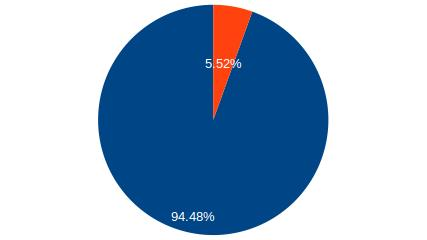
\includegraphics[width=0.5\textwidth]{./images/md18fevr}}~~
\subfloat[Left mandibles]{\label{figmg18fevr}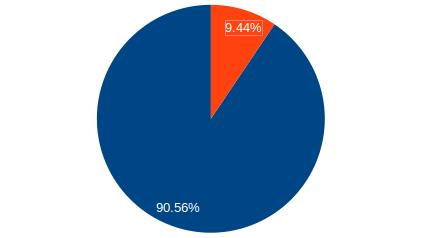
\includegraphics[width=0.5\textwidth]{./images/mg18fevr}}
\caption{Success rates of estimating landmarks on mandibles}
\label{figm18fevr}
\end{figure}~\\
In a different side, if we have statistics on each set of mandible, the success rates of left mandible are \textit{87.18\%} for sub-set 1 and \textit{97.80\%} for sub-set 2 (figure \ref{figmg18fevr}). For right mandible are \textit{94.52\%} and \textit{94.37\%} for sub-set 1 and sub-set 2, respective (figure \ref{figmd18fevr}).
\begin{figure}[h!]
\centering
\subfloat[Sub-set 1]{\label{figmg18fevrS1}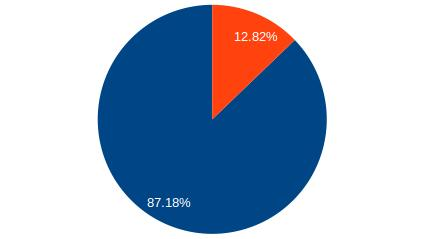
\includegraphics[width=0.5\textwidth]{./images/mg18fevrSize1}}~~
\subfloat[Sub-set 2]{\label{figmg18fevrS2}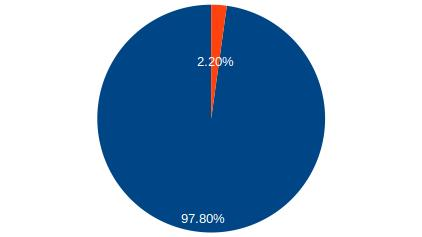
\includegraphics[width=0.5\textwidth]{./images/mg18fevrSize2}}
\caption{Success rates of estimating landmarks on each sub-set of left mandibles}
\label{figmg18fevr}
\end{figure}~\\
\begin{figure}[h!]
\centering
\subfloat[Sub-set 1]{\label{figmd18fevrS1}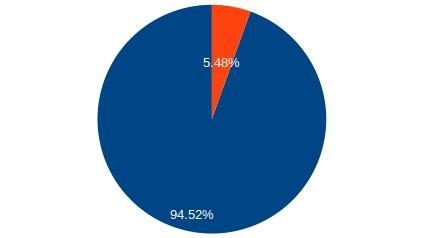
\includegraphics[width=0.5\textwidth]{./images/md18fevrSize1}}~~
\subfloat[Sub-set 2]{\label{figmd18fevrS2}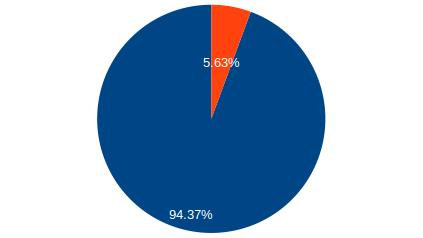
\includegraphics[width=0.5\textwidth]{./images/md18fevrSize2}}
\caption{Success rates of estimating landmarks on each sub-set of right mandibles}
\label{figmd18fevr}
\end{figure}~\\
Although the result from the method is good but it depends much on the result of segmentation. If the segmentation is not good and have many noises, the result of the method will be affected.

\subsection{Singular value decomposition (SVD)}
The PCA method is more effected by the noise, instead of using all the curve points, SVD just using a subset of points by optimal alignment between corresponding points of model and scene. Assume that \texttt{M} is a subset of the model points, \textbf{S} is a subset of the scene points and $p_i \in M, q_i \in S$ are two corresponding points. We would like to find the matrix transformed \textbf{R} so that the pair-wise distances between the corresesponding points is minimum. The pairwise distance is indicated by equation (\ref{eqpwdistance}).
\begin{center}
\begin{equation}\label{eqpwdistance}
	E = \sum_{i=1}^{n} {\|q_i - p_i^{'}\|}
\end{equation}
\end{center}
Where:
\begin{itemize}
	\item \textit{n}: is number of corresponding points
	\item \textit{$q_i$}: point of scene
	\item \textit{$p_i^{'}$}: point of model which corresponding with \texttt{$q_i$}
\end{itemize}
In detail, SVD method includes the following steps:
\begin{itemize}
	\item Calculate the cross covariance matrix: $M = P.Q^T$, where $P(Q)$ are matrix with i-th column is vector $p_i - c_T$ ($q_i - c_S$),
	\item Compute the singular value decomposition of matrix $M$: \textbf{$M = U.W.V^T$}. Where:
	\begin{itemize}
		\item U,V are \textit{m} x \textit{m} orthonormal matrices
		\item W is a diagonal \textit{m} x \textit{m} matrix with non-negative entries.
	\end{itemize}
	\item Indicate the orthonormal matrix (rotation matrix) $R = V.U^T$
\end{itemize}
\subsubsection{Result}
SVD method is solving the noise problem of PCA by using a set of corresponding points. The result obtained by applying the SVD also better PCA. But a disadvantage of SVD is requiring a accurate correspondences set of points which are usually not available.
\subsection{Iterative closest point (ICP)}
Based on the advantage and disadvantage of PCA and SVD. ICP combines two previous methods. The idea of ICP is using PCA to intial guess of correspondences and repeating SVD to improve correspondences. The steps of ICP are:
\begin{itemize}
	\item Transform the model by PCA aligment
	\item For each transformed model point, assign the closest scene point as its corresponding point. Align model and scene by SVD
	\item Repeat the step (2) until a termination criteria is met.
\end{itemize}
\section{Patch-based}
In recent year, beyond using the pixels to extract and compare the features of the images, patch-based is more and more catch on because the advantages of processing time and less memory use of program. The behind idea of this technique is extracting all patches (with(out) overlap) on the input image. The size of the patches are fixed and smaller than the size of the image. Most of the methods with patch-based spend more time to extract and compare the relation between them. In this section, we will mention to comparing methods between patches; next, some processing methods on patches are introduced; finally, we want to present some application based on patch-base. During this section, we will use some notations as follows: \textbf{Z, X} are source and target image; \textbf{M, N} are two patches on Z and X with the size \textit{nxn}.
\subsection{Comparing method between patches}
In this part, we will mention to the methods which are used to measure distance between two patches \textit{M} and \textit{N}.
\subsubsection{Pixel-based distance(L1 distance)}
The similarity measure between patches is determined by sum of the distance between each pair of pixels in the patches.
\begin{equation}\label{l1}
	d(M,N) = \sum_d(M_d - N_d)
\end{equation}
Where: \textit{d} is the pixels on patches.\\[0.2cm]
However, L1 distance (equation \ref{l1}) is very sensitive with the changing of pixels such as rotation, translation or scale. Instead of using the L1 distance, we can use another norm (L2 distance) on the pixels as:
\begin{equation}\label{l2}
	d(M,N) = \sum_d(M_d - N_d)^2
\end{equation}
\subsubsection{Correlation}
\begin{equation}\label{correlation}
	d(M,N) = \frac{\sum_d(M_d - \overline{M_d})(N_d - \overline{N_d})}{\sigma_1.\sigma_2}
\end{equation}
Where: $\overline{x_i}, \sigma_i$ is the mean and standard deviation of the pixels on patch $x_i$.
\subsubsection{Descriptor distance}
In this way, the characteristic of the patch is presented into other dimension spatial (i.e vector). Then, the measure distance between two patches will be moved to distance between two descriptors.
\subsubsection{Probabilistic matching}
In this case, we do not measure the distance between patches directly. Instead, we calculate the probability to the patches \textbf{M, N} is belong to the same group.
\subsection{Methods on patches}
This section, we will investigates recent articles that follow these themes. Most of patch-based methods can be divided into three groups: in the first group, the feature on patches is presented into other dimensional and comparing \cite{bentley1975multidimensional, sproull1991refinements, niyogi1996example, kumar2008good}; the second group includes the methods that directly compare the pixels in the patches \cite{barnes2010generalized, barnes2009patchmatch, xiao2011fast}; the last group is used dictionary to compare the patches\cite{datar2004locality}.\\[0.2cm]
The first group, we have to say about the \textit{kd-tree} (k is the number of dimension in tree). This method is introduced by \cite{bentley1975multidimensional}. Bentley used the binary tree to present the relationship between the records in a file. Firstly, attributes of the record is presented to other data in other dimensional (vector). Then, the datas is used to construct a binary tree. And patch matching will be done in this tree. In this method, we can spend more time and cost to build the tree but we can reduce the cost during searching a patch. Based on the idea of kd-tree, Sproull and Robert propose PCA-tree \cite{sproull1991refinements}. The idea of this medthod is reduce the number of dimension of data by using eigenvector and eigenvalue of patches. Besides, we have also the methods based on the tree as TSVQ \cite{niyogi1996example} or vp-tree\cite{kumar2008good}.\\[0.2cm]
In the scheme of methods which based on comparing of pixels in the patches. Connelly\cite{barnes2009patchmatch} was given the concepts of Nearest Neighbor Field (NNF) to compare the distance between two patches by using a function $f: S \rightarrow R^2$. This method includes 2 steps: (1) the matching patches is randomly initialization with NNF; (2) an iteration of propagation and randomization is applied to determine the best patch match for searching patch. In a different side, instead finding the best matching of a patch, we would like to have a set of patches that matching with the searching patch\cite{barnes2010generalized}. In this method, they try to extend on patch matching include k-nearest neighbors, the matching is done through rotation, scale and matching descriptor. They also mention a new search strategy, called ``enrichment" and parallel searching based on multiple core of GPU. Besides, Xiao\cite{xiao2011fast} propose a method that the authors evalutate this is a fast method. Xiao's method refers to move and calculate the distance between the patches. It was also improved by reducing the complexity of the calculating distance of patches.\\[0.2cm]
The last group on patch-based is used dictionary such as Locality Sensitive Hashing (LSH)\cite{datar2004locality}. Firstly, the dimension of each patch is reduced and stored into \textbf{PatchTable}. Follow with this way, the similar patches will be stored into a record in PatchTable. Patch-matching is finished by checking each cell in PatchTable with searching patch to indicate the best matching location.
\subsection{Application on patches}
Patch-based is widely used in 2D, 3D images and video application \cite{barnessurvey}. This section will introduce some domain in 2D image where we can apply the patch-based.
\subsubsection{Inpainting and reshuffling}
Image inpainting \cite{guillemot2014image} image is technique that removes a region (foreground) in the image by replacing it with other region(background) in the image. The backround can be extract from this image or from another image. Meanwhile, reshuffling \cite{cho2008patch} is moving a region to new postion in the image. The aim of this work is create a new image consistent with the user constraints. Image reshuffling can be treated as an extension of image inpainting by initializing the regions to be synthesized by user specified contents.
\subsubsection{Denoising}
Image denoising\cite{barnes2010generalized} is popular application of patch-based (i.e Gaussian filter, Sobel filter). A patch is moved over the pixels of image. At each position, a weighted average is calculated to denoise the pixels.